\documentclass[12pt, titlepage]{article}

\usepackage{fullpage}
\usepackage[round]{natbib}
\usepackage{multirow}
\usepackage{multicol}
\usepackage{booktabs}
\usepackage{tabularx}
\usepackage{graphicx}
\usepackage{float}
\usepackage{hyperref}
\hypersetup{
    colorlinks,
    citecolor=blue,
    filecolor=black,
    linkcolor=red,
    urlcolor=blue
}

%% Comments

\usepackage{color}

\newif\ifcomments\commentstrue %displays comments
%\newif\ifcomments\commentsfalse %so that comments do not display

\ifcomments
\newcommand{\authornote}[3]{\textcolor{#1}{[#3 ---#2]}}
\newcommand{\todo}[1]{\textcolor{red}{[TODO: #1]}}
\else
\newcommand{\authornote}[3]{}
\newcommand{\todo}[1]{}
\fi

\newcommand{\wss}[1]{\authornote{blue}{SS}{#1}} 
\newcommand{\plt}[1]{\authornote{magenta}{TPLT}{#1}} %For explanation of the template
\newcommand{\an}[1]{\authornote{cyan}{Author}{#1}}

%% Common Parts

\newcommand{\progname}{ProgName} % PUT YOUR PROGRAM NAME HERE
\newcommand{\authname}{Team \#, Team Name
\\ Student 1 name
\\ Student 2 name
\\ Student 3 name
\\ Student 4 name} % AUTHOR NAMES                  

\usepackage{hyperref}
    \hypersetup{colorlinks=true, linkcolor=blue, citecolor=blue, filecolor=blue,
                urlcolor=blue, unicode=false}
    \urlstyle{same}
                                


\newcounter{acnum}
\newcommand{\actheacnum}{AC\theacnum}
\newcommand{\acref}[1]{AC\ref{#1}}

\newcounter{ucnum}
\newcommand{\uctheucnum}{UC\theucnum}
\newcommand{\uref}[1]{UC\ref{#1}}

\newcounter{mnum}
\newcommand{\mthemnum}{M\themnum}
\newcommand{\mref}[1]{M\ref{#1}}

\begin{document}

\title{Module Guide for \progname{}} 
\author{\authname}
\date{\today}

\maketitle

\pagenumbering{roman}

\section{Revision History}

\begin{tabularx}{\textwidth}{p{3cm}p{2cm}X}
\toprule {\bf Date} & {\bf Version} & {\bf Notes}\\
\midrule
01/11/2024 & 0.0 & Initial Document \\
01/12/2024 & 0.1 & Initial Draft of Anticipated and Unlikely Changes and
  Module Hierarchy sections; Added some terms to Abbreviations and Acronyms
  section \\
01/13/2024 & 0.2 & Added Uses Hierarchy among modules diagram \\
01/14/2024 & 0.3 & Filled out Traceability Matrices for Traceability Matrix
  section \\
01/15/2024 & 0.4 & Made small edits to Table 1 in Module Hierarchy section and
  Table 4 in Traceability Matrix section; Initial Draft of Module
  Decomposition section completed \\
\bottomrule
\end{tabularx}

\newpage

\section{Reference Material}

This section records information for easy reference.

\subsection{Abbreviations and Acronyms}

\renewcommand{\arraystretch}{1.2}
\begin{tabular}{l l} 
  \toprule		
  \textbf{symbol} & \textbf{description} \\
  \midrule 
  AC & Anticipated Change \\
  AI/ML & Artificial Intelligence/Machine Learning \\
  DAG & Directed Acyclic Graph \\
  \multirow{3}{*}{DICOM} & Digital Imaging and Communications in Medicine; \\
  & technical standard for digital storage/transmission \\
  & of medical images and related information \\
  GUI & Graphical User Interface \\
  \multirow{2}{*}{JPEG/JPG} & Joint Photographic Experts Group; digital image \\
  & compression standard, image format \\
  M & Module \\
  MG & Module Guide \\
  MVC & Model-View-Controller Software Architecture \\
  NLP & Natural Language Processing \\
  OS & Operating System \\
  R & Requirement \\
  SC & Scientific Computing \\
  SRS & Software Requirements Specification \\
  \multirow{3}{*}{\progname} & The Process of Designing and Developing Software; \\
  & a reference to the software application described \\
  & in this document \\
  UC & Unlikely Change \\
  \bottomrule
\end{tabular}\\

\newpage

\tableofcontents

\listoftables

\listoffigures

\newpage

\pagenumbering{arabic}

\section{Introduction}

Decomposing a system into modules is a commonly accepted approach to developing
software.  A module is a work assignment for a programmer or programming
team~\citep{ParnasEtAl1984}.  We advocate a decomposition
based on the principle of information hiding~\citep{Parnas1972a}.  This
principle supports design for change, because the ``secrets'' that each module
hides represent likely future changes.  Design for change is valuable in SC,
where modifications are frequent, especially during initial development as the
solution space is explored.  

Our design follows the rules layed out by \citet{ParnasEtAl1984}, as follows:
\begin{itemize}
\item System details that are likely to change independently should be the
  secrets of separate modules.
\item Each data structure is implemented in only one module.
\item Any other program that requires information stored in a module's data
  structures must obtain it by calling access programs belonging to that module.
\end{itemize}

After completing the first stage of the design, the Software Requirements
Specification (SRS), the Module Guide (MG) is developed~\citep{ParnasEtAl1984}. The MG
specifies the modular structure of the system and is intended to allow both
designers and maintainers to easily identify the parts of the software.  The
potential readers of this document are as follows:

\begin{itemize}
\item New project members: This document can be a guide for a new project member
  to easily understand the overall structure and quickly find the
  relevant modules they are searching for.
\item Maintainers: The hierarchical structure of the module guide improves the
  maintainers' understanding when they need to make changes to the system. It is
  important for a maintainer to update the relevant sections of the document
  after changes have been made.
\item Designers: Once the module guide has been written, it can be used to
  check for consistency, feasibility, and flexibility. Designers can verify the
  system in various ways, such as consistency among modules, feasibility of the
  decomposition, and flexibility of the design.
\end{itemize}

The rest of the document is organized as follows. Section
\ref{SecChange} lists the anticipated and unlikely changes of the software
requirements. Section \ref{SecMH} summarizes the module decomposition that
was constructed according to the likely changes. Section \ref{SecConnection}
specifies the connections between the software requirements and the
modules. Section \ref{SecMD} gives a detailed description of the
modules. Section \ref{SecTM} includes two traceability matrices. One checks
the completeness of the design against the requirements provided in the SRS. The
other shows the relation between anticipated changes and the modules. Section
\ref{SecUse} describes the use relation between modules.

\section{Anticipated and Unlikely Changes} \label{SecChange}

This section lists possible changes to the system. According to the likeliness
of the change, the possible changes are classified into two
categories. Anticipated changes are listed in Section \ref{SecAchange}, and
unlikely changes are listed in Section \ref{SecUchange}.

\subsection{Anticipated Changes} \label{SecAchange}

Anticipated changes are the source of the information that is to be hidden
inside the modules. Ideally, changing one of the anticipated changes will only
require changing the one module that hides the associated decision. The approach
adapted here is called design for
change.

\begin{description}
  \begin{item}[\refstepcounter{acnum} \actheacnum \label{acHardware}:]
    The specific hardware on which the software is running.
  \end{item}
  \begin{item}[\refstepcounter{acnum} \actheacnum \label{acDiseases}:]
    The specific selection of diseases that the AI/ML model will look for when
    performing the chest x-ray scan/read.
  \end{item}
  \begin{item}[\refstepcounter{acnum} \actheacnum \label{acRadReport}:]
    The output radiology report generated using NLP (progressing from report
    components to more complete report).
  \end{item}
  \begin{item}[\refstepcounter{acnum} \actheacnum \label{acAppGUI}:]
    The various application pages/GUI (page layout changes/redesign, etc.).
  \end{item}
  \begin{item}[\refstepcounter{acnum} \actheacnum \label{acMedInstInterf}:]
    The module for interfacing with the IT system(s) of the medical
    institution(s) using this application.
  \end{item}
\end{description}

\subsection{Unlikely Changes} \label{SecUchange}

The module design should be as general as possible. However, a general system is
more complex. Sometimes this complexity is not necessary. Fixing some design
decisions at the system architecture stage can simplify the software design. If
these decision should later need to be changed, then many parts of the design
will potentially need to be modified. Hence, it is not intended that these
decisions will be changed.

\begin{description}
  \begin{item}[\refstepcounter{ucnum} \uctheucnum \label{ucIO}:]
    Input/Output devices (Input: File and/or Keyboard, Output: File, Memory,
    and/or Screen).
  \end{item}
  \begin{item}[\refstepcounter{ucnum} \uctheucnum \label{ucModelLib}:]
    The same (Python) library/libraries will be used for the AI/ML model.
  \end{item}
  \begin{item}[\refstepcounter{ucnum} \uctheucnum \label{ucUserAuth}:]
    The database/backend provider (Firebase) will be used for user
    authentication/management and application security.
  \end{item}
  \begin{item}[\refstepcounter{ucnum} \uctheucnum \label{ucBackend}:]
    The same backend/database provider (Firebase) will be used.
  \end{item}
  \begin{item}[\refstepcounter{ucnum} \uctheucnum \label{ucInputFormat}:]
    The input format of the chest x-ray data (DICOM) into the application.
  \end{item}
  \begin{item}[\refstepcounter{ucnum} \uctheucnum \label{ucModelLib}:]
    The input format of the chest x-ray image (JPG or JPEG) into the AI/ML
    model for performing the chest x-ray scan/read.
  \end{item}
\end{description}

\section{Module Hierarchy} \label{SecMH}

This section provides an overview of the module design. Modules are summarized
in a hierarchy decomposed by secrets in Table \ref{TblMH}. The modules listed
below, which are leaves in the hierarchy tree, are the modules that will
actually be implemented.

\begin{multicols}{2}
\begin{description}
  \item [\refstepcounter{mnum} \mthemnum \label{mAIModel}:] AIModel Module
  \item [\refstepcounter{mnum} \mthemnum \label{mChXRR}:] ChestXRayRead Module
  \item [\refstepcounter{mnum} \mthemnum \label{mResGen}:] ResultsGen Module
  \item [\refstepcounter{mnum} \mthemnum \label{mNLPModel}:] NLPModel Module
  \item [\refstepcounter{mnum} \mthemnum \label{mRepCompGen}:] RepCompGen Module
  \item [\refstepcounter{mnum} \mthemnum \label{mBackend}:] Backend Module
  \item [\refstepcounter{mnum} \mthemnum \label{mDatabaseOps}:] DatabaseOps Module
  \item [\refstepcounter{mnum} \mthemnum \label{mUserAuthMgmt}:] UserAuthMgmt Module
  \item [\refstepcounter{mnum} \mthemnum \label{mMedInstInter}:] MedInstInter Module
  \item [\refstepcounter{mnum} \mthemnum \label{mAppController}:] AppController Module
  \item [\refstepcounter{mnum} \mthemnum \label{mAppGUI}:] AppGUI Module
  \item [\refstepcounter{mnum} \mthemnum \label{mLogin}:] Login Module
  \item [\refstepcounter{mnum} \mthemnum \label{mPerfScan}:] PerfScan Module
  \item [\refstepcounter{mnum} \mthemnum \label{mViewResults}:] ViewResults Module
\end{description}
\end{multicols}

\begin{table}[H]
  \centering
  \begin{tabular}{p{0.3\textwidth} p{0.6\textwidth}}
    \toprule
    \textbf{Level 1} & \textbf{Level 2} \\
    \midrule

    {Hardware-Hiding Module} & MedInstInter \\
    \midrule

    \multirow{8}{0.3\textwidth}{Behaviour-Hiding Module} & ChestXRayRead \\
    & ResultsGen \\
    & RepCompGen \\
    & DatabaseOps \\
    & UserAuthMgmt \\
    & Login \\ 
    & PerfScan \\
    & ViewResults \\
    \midrule

    \multirow{5}{0.3\textwidth}{Software Decision Module} & AIModel \\
    & NLPModel \\
    & Backend \\
    & AppController \\
    & AppGUI \\
    \bottomrule

  \end{tabular}
  \caption{Module Hierarchy}
  \label{TblMH}
\end{table}

The modules listed above are also organized following an overall MVC software
architecture for this application. This MVC-oriented organization is shown
below in Table \ref{TblMMH}.

\begin{table}[H]
  \centering
  \begin{tabular}{p{0.3\textwidth} p{0.6\textwidth}}
    \toprule
    \textbf{Level 1} & \textbf{Level 2} \\
    \midrule

    \multirow{6}{0.3\textwidth}{Model Module} & ChestXRayRead \\
    & ResultsGen \\
    & RepCompGen \\
    & DatabaseOps \\
    & UserAuthMgmt \\
    & MedInstInter \\
    \midrule

    \multirow{3}{0.3\textwidth}{View Module} & Login \\ 
    & PerfScan \\
    & ViewResults \\
    \midrule

    \multirow{5}{0.3\textwidth}{Controller Module} & AIModel \\
    & NLPModel \\
    & Backend \\
    & AppController \\
    & AppGUI \\
    \bottomrule

  \end{tabular}
  \caption{Module MVC Hierarchy}
  \label{TblMMH}
\end{table}

\section{Connection Between Requirements and Design} \label{SecConnection}

The design of the system is intended to satisfy the requirements developed in
the SRS. In this stage, the system is decomposed into modules. The connection
between requirements and modules is listed in Table~\ref{TblRT}.

\section{Module Decomposition} \label{SecMD}

Modules are decomposed according to the principle of ``information hiding''
proposed by \citet{ParnasEtAl1984}. The \emph{Secrets} field in a module
decomposition is a brief statement of the design decision hidden by the
module. The \emph{Services} field specifies \emph{what} the module will do
without documenting \emph{how} to do it. For each module, a suggestion for the
implementing software is given under the \emph{Implemented By} title. If the
entry is \emph{OS}, this means that the module is provided by the operating
system or by standard programming language libraries.  \emph{\progname{}} means the
module will be implemented by the \progname{} software.

Only the leaf modules in the hierarchy have to be implemented. If a dash
(\emph{--}) is shown, this means that the module is not a leaf and will not have
to be implemented.

\subsection{Hardware Hiding Module}

\begin{description}
\item[Secrets:] The data structure and algorithm used to implement the virtual
  hardware.
\item[Services:] Serves as a virtual hardware used by the rest of the
  system. This module provides the interface between the hardware and the
  software. So, the system can use it to display outputs or to accept inputs.
\item[Implemented By:] OS
\end{description}

\subsubsection{MedInstInter Module (\mref{mMedInstInter})}

\begin{description}
\item[Secrets:] The data structures and algorithms used to interface with
  the IT system(s) of the medical institution(s).
\item[Services:] Serves as an interface to transfer information between the
  medical institution(s)' IT system(s) and the application.
\item[Implemented By:] [Your Program Name Here]
\end{description}

\subsection{Behaviour-Hiding Module}

\begin{description}
\item[Secrets:] The contents of the required behaviours.
\item[Services:] Includes programs that provide externally visible behaviour
  of the system as specified in the software requirements specification (SRS)
  documents. This module serves as a communication layer between the
  hardware-hiding module and the software decision module. The programs in
  this module will need to change if there are changes in the SRS.
\item[Implemented By:] --
\end{description}

\subsubsection{ChestXRayRead Module (\mref{mChXRR})}

\begin{description}
\item[Secrets:] The chest x-ray reader data structure(s) and algorithm(s)
  used to scan a chest x-ray image and look for/detect the possible presence
  of certain diseases/infections (after converting from DICOM to JPEG).
\item[Services:] Reads/scans the chest x-ray image, performs some analysis and
  returns the processed disease/infection probability data.
\item[Implemented By:] [Your Program Name Here]
\item[Type of Module:] Library
\end{description}

\subsubsection{ResultsGen Module (\mref{mResGen})}

\begin{description}
\item[Secrets:] The data structure(s) and algorithm(s) used to further
  process, interpret and store the results generated from scanning the chest
  x-ray image.
\item[Services:] Process ChestXRayRead Module output, interpret the processed
  disease/infection probability data and return generated results for use in
  generating the radiology report (components).
\item[Implemented By:] [Your Program Name Here]
\item[Type of Module:] Library, Abstract Object
\end{description}

\subsubsection{RepCompGen Module (\mref{mRepCompGen})}

\begin{description}
\item[Secrets:] The data structure(s) and algorithm(s) (including NLP) used to
  generate the radiology report (components) using the chest x-ray read/scan
  results.
\item[Services:] Take the AIModel Module output and generate the radiology
  report (components) documenting the results/predictions from analyzing the
  chest x-ray image using natural language.
\item[Implemented By:] [Your Program Name Here]
\item[Type of Module:] Library, Abstract Object
\end{description}

\subsubsection{DatabaseOps Module (\mref{mDatabaseOps})}

\begin{description}
\item[Secrets:] The data structure(s) and algorithm(s) used to organize, store
  and retrieve patient data and application user data.
\item[Services:] Organizes, stores and retrieves patient data from the 
  database. Also manages the chest x-ray image and scan results and 
  predictions for each patient. Does likewise for application user data.
\item[Implemented By:] [Your Program Name Here]
\item[Type of Module:] Record, Library, Abstract Object
\end{description}

\subsubsection{UserAuthMgmt Module (\mref{mUserAuthMgmt})}

\begin{description}
\item[Secrets:] The data structure(s) and algorithm(s) used to authenticate
  and manage application users.
\item[Services:] Protects patient data by only granting access to
  authenticated application users. Also manages users (i.e. add/remove users).
\item[Implemented By:] [Your Program Name Here]
\item[Type of Module:] Library, Abstract Object
\end{description}

\subsubsection{Login Module (\mref{mLogin})}

\begin{description}
\item[Secrets:] The data structure(s) and algorithm(s) used to show and make
  functional the login functionality for users.
\item[Services:] Displays login portal and authenticates user logins into this
  application.
\item[Implemented By:] [Your Program Name Here]
\item[Type of Module:] Library, Abstract Object
\end{description}

\subsubsection{PerfScan Module (\mref{mPerfScan})}

\begin{description}
\item[Secrets:] The data structure(s) and algorithm(s) used to show and make
  functional the chest x-ray read/scan functionality for users.
\item[Services:] Displays portal for users to submit chest x-ray images for
  read/scan to get disease/infection predictions.
\item[Implemented By:] [Your Program Name Here]
\item[Type of Module:] Library, Abstract Object
\end{description}

\subsubsection{ViewResults Module (\mref{mViewResults})}

\begin{description}
\item[Secrets:] The data structure(s) and algorithm(s) used to show and make
  functional the view results functionality for users.
\item[Services:] Displays the results of the (latest) chest x-ray read/scan
  for a given patient to the user (i.e. displays the latest radiology report).
\item[Implemented By:] [Your Program Name Here]
\item[Type of Module:] Library, Abstract Object
\end{description}

\subsection{Software Decision Module}

\begin{description}
\item[Secrets:] The design decision based on mathematical theorems, physical
  facts, or programming considerations. The secrets of this module are
  \emph{not} described in the SRS.
\item[Services:] Includes data structure and algorithms used in the system that
  do not provide direct interaction with the user. 
  % Changes in these modules are more likely to be motivated by a desire to
  % improve performance than by externally imposed changes.
\item[Implemented By:] --
\end{description}

\subsubsection{AIModel Module (\mref{mAIModel})}

\begin{description}
\item[Secrets:] The data structure(s) and algorithm(s) used (including in
  Modules \mref{mChXRR} ChestXRayRead and \mref{mResGen} ResultsGen) to
  read/scan chest x-ray images and interpret the disease/infection probability
  results. The ROC values used to interpret the disease/infection probability
  results and give predictions.
\item[Services:] Reads/scans chest x-ray images, interpret the data and return
  disease/infection predictions.
\item[Implemented By:] [Your Program Name Here]
\item[Type of Module:] Library, Abstract Object
\end{description}

\subsubsection{NLP Module (\mref{mNLPModel})}

\begin{description}
\item[Secrets:] The data structure(s) and algorithm(s) used (including in
  Module \mref{mRepCompGen} RepCompGen) to generate a natural language
  radiology report to document the results and predictions of the chest x-ray
  read/scan.
\item[Services:] Generates the readiology report documenting the results and
  predictions of the chest x-ray read/scan using natural language.
\item[Implemented By:] [Your Program Name Here]
\item[Type of Module:] Library, Abstract Object
\end{description}

\subsubsection{Backend Module (\mref{mBackend})}

\begin{description}
\item[Secrets:] The data structure(s) and algorithm(s) used (including in
  Modules \mref{mDatabaseOps} DatabaseOps, \mref{mUserAuthMgmt} UserAuthMgmt
  and \mref{mMedInstInter} MedInstInter) to manage and protect patient data,
  authenticate users and interface with external IT system(s) securely.
\item[Services:] Organize, store and retrieve patient data, protect patient
  data integrity and privacy by authenticating application users before
  granting access to sensitive information. Interface with IT system(s) of
  medical institutions to transfer/retrieve patient data securely.
\item[Implemented By:] [Your Program Name Here]
\item[Type of Module:] Record, Library, Abstract Object
\end{description}

\subsubsection{AppController Module (\mref{mAppController})}

\begin{description}
\item[Secrets:] The interactions and inter-dependencies of all other software
  decision modules (\mref{mAIModel} AIModel, \mref{mNLPModel} NLPModel,
  \mref{mBackend} Backend and \mref{mAppGUI} AppGUI) of this application.
\item[Services:] Enables the users to submit chest x-ray images, performs
  scans/reads of those images and produces disease/infection predictions that
  are documented in (a) natural language radiology report (components).
\item[Implemented By:] [Your Program Name Here]
\item[Type of Module:] Library
\end{description}

\subsubsection{AppGUI Module (\mref{mAppGUI})}

\begin{description}
\item[Secrets:] The data structure(s) and algorithm(s) used (including in
  Modules \mref{mLogin} Login, \mref{mPerfScan} PerfScan and
  \mref{mViewResults}) to show application functionalities to the users,
  accept user inputs and show outputs.
\item[Services:] Show application functionalities to the users in a
  GUI, accept user inputs (i.e. chest x-ray images) and show outputs (i.e.
  predictions and radiology report/components).
\item[Implemented By:] [Your Program Name Here]
\item[Type of Module:] Library
\end{description}

\section{Traceability Matrix} \label{SecTM}

This section shows two traceability matrices: between the modules and the
requirements and between the modules and the anticipated changes.

% the table should use mref, the requirements should be named, use something
% like fref
\begin{table}[H]
\centering
\begin{tabular}{p{0.2\textwidth} p{0.6\textwidth}}
\toprule
\textbf{Req.} & \textbf{Modules} \\
\midrule
FR1 & \mref{mChXRR}, \mref{mPerfScan} \\
FR2 & \mref{mChXRR}, \mref{mPerfScan} \\
FR3 & \mref{mResGen}, \mref{mViewResults} \\
FR4 & \mref{mResGen}, \mref{mDatabaseOps}, \mref{mViewResults} \\
FR5 & \mref{mDatabaseOps}, \mref{mAppGUI} \\
FR6 & \mref{mAIModel} \\
FR7 & \mref{mMedInstInter}, \mref{mAppController}, \mref{mAppGUI} \\
FR8 & \mref{mChXRR} \\
FR9 & \mref{mBackend}, \mref{mDatabaseOps} \\
FR10 & \mref{mUserAuthMgmt}, \mref{mLogin} \\
FR11 & \mref{mAppController}, \mref{mAppGUI}, \mref{mViewResults} \\
\bottomrule
\end{tabular}
\caption{Trace Between Requirements and Modules}
\label{TblRT}
\end{table}

\begin{table}[H]
\centering
\begin{tabular}{p{0.2\textwidth} p{0.6\textwidth}}
\toprule
\textbf{AC} & \textbf{Modules} \\
\midrule
\acref{acHardware} & \mref{mAIModel}, \mref{mChXRR}, \mref{mResGen},
  \mref{mNLPModel}, \mref{mRepCompGen}, \mref{mBackend}, \mref{mDatabaseOps},
  \mref{mUserAuthMgmt}, \mref{mMedInstInter}, \mref{mAppController},
  \mref{mAppGUI}, \mref{mLogin}, \mref{mPerfScan}, \mref{mViewResults} \\
\acref{acDiseases} & \mref{mAIModel} \\
\acref{acRadReport} & \mref{mNLPModel} \\
\acref{acAppGUI} & \mref{mAppGUI} \\
\acref{acMedInstInterf} & \mref{mMedInstInter} \\
\bottomrule
\end{tabular}
\caption{Trace Between Anticipated Changes and Modules}
\label{TblACT}
\end{table}

\section{Use Hierarchy Between Modules} \label{SecUse}

In this section, the uses hierarchy between modules is
provided. \citet{Parnas1978} said of two programs A and B that A {\em uses} B if
correct execution of B may be necessary for A to complete the task described in
its specification. That is, A {\em uses} B if there exist situations in which
the correct functioning of A depends upon the availability of a correct
implementation of B.  Figure \ref{FigUH} illustrates the use relation between
the modules. It can be seen that the graph is a directed acyclic graph
(DAG). Each level of the hierarchy offers a testable and usable subset of the
system, and modules in the higher level of the hierarchy are essentially simpler
because they use modules from the lower levels.

\begin{figure}[H]
\centering
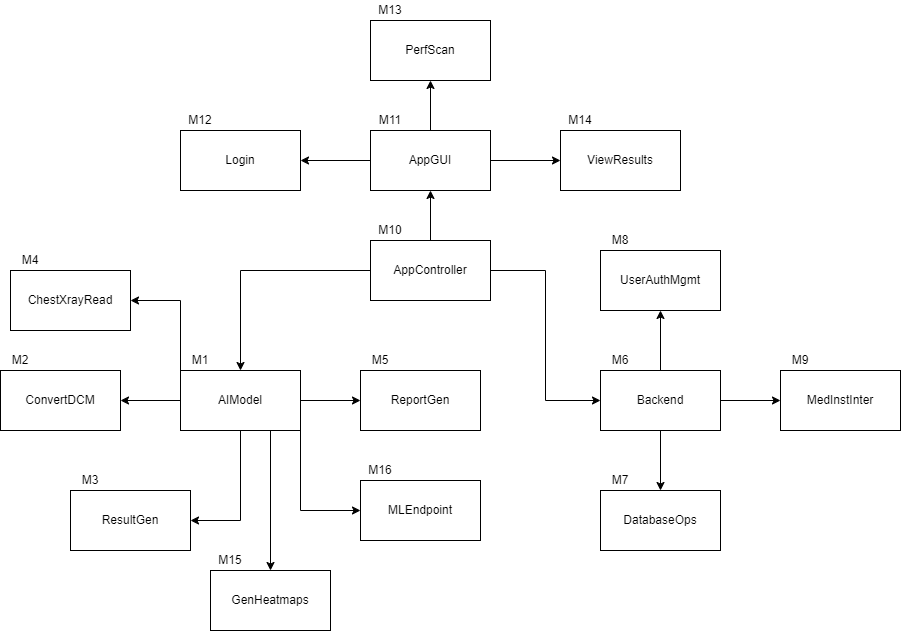
\includegraphics[width=0.7\textwidth]{UsesHierarchy.png}
\caption{Use hierarchy among modules}
\label{FigUH}
\end{figure}

%\section*{References}

\bibliographystyle {plainnat}
\bibliography{../../../refs/References}

\newpage{}

\end{document}